\zchapter{Your Account}\label{SetupAccount}

% How to actually make an account. Most Freshers never do this :-(

%\begin{mdframed}

\section{Getting it}

\textsc{signing up at the O'Day stall does not give you access to all of UCC's services. You need to create an account at the UCC clubroom.}

Your UCC account is \emph{the} most important thing you can have as a member. In addition to providing a way for us to communicate with you, the account lets you log into any of our clubroom machines, as well as granting you access to our user servers, wireless network, online drink and snack machines, and more.

Once you're at the clubroom and ready to create an account, ask around for a Wheel or Committee member and have your membership sticker (we normally put it on your student card on O-Day) to set up your account. You'll need a user name and a password to memorise, but it's a pretty simple procedure once you've found the right person!


Now that you have an account, you can use it to log into any of our clubroom machines. If you want to log onto one of our servers, you'll need to use the SSH program. If you're having trouble, just ask someone in the clubroom --- we don't \pun{byte}!

Changing your UCC password can either be done by Ctrl-Alt-Del on a windows machine or using the command \shell{passwd} on a Linux/Unix machine.
Accessing the UCC WiFi network can be a bit tricky (particularly on Windows machines). Ask someone if you need help, or refer to \url{http://wiki.ucc.asn.au/Wifi}

%\end{mdframed}

%\begin{mdframed}

\section{SSH for Great Good}

SSH is a program that lets you remotely access UCC's servers. These can be used for almost anything (legal) you can imagine; programming, website hosting, file storage, IRC chatting, dispensing drinks, and many more things.

The easiest way to use SSH is from a Linux clubroom desktop. Simply open a "terminal" application, type "ssh ssh" and enter your password.

From a windows machine, open a program called "PuTTy" (or "KiTTy" on some machines). Enter the address "ssh" and click "Open".

Once you are logged in, a good way to start is running "irssi -c irc" and then typing "/join \#ucc". The interface of irssi takes some getting used to, but when combined with "screen" (ask someone for help) it is a powerful weapon for procrastination.

You don't have to be in the UCC clubroom to use SSH! Simply use "username@ssh.ucc.asn.au" as the address to connect to.

%\begin{figure}[H]
%	\centering
%	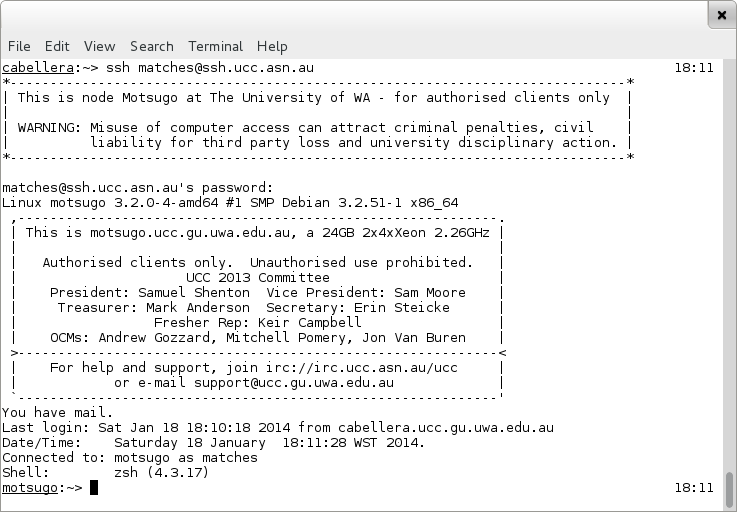
\includegraphics[width=1.0\textwidth]{figures/ssh.png}
%	\caption{SSH from Linux} 
%	\label{ssh.png}
%\end{figure}

%\begin{figure}[H]
%	\centering
%	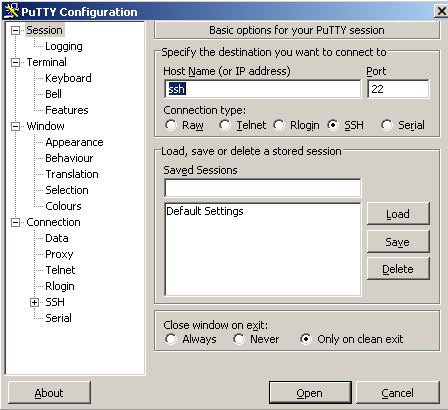
\includegraphics[width=0.5\textwidth]{figures/putty.png}
%	\caption{Use PuTTY to SSH. Just press "Open"} 
%	\label{putty.png}
%\end{figure}

%\end{mdframed}
